%%%%%%%%%%%%%%%%%%%% book.tex %%%%%%%%%%%%%%%%%%%%%%%%%%%%%
%
% sample root file for the chapters of your "monograph"
%
% Use this file as a template for your own input.
%
%%%%%%%%%%%%%%%% Springer-Verlag %%%%%%%%%%%%%%%%%%%%%%%%%%


% RECOMMENDED %%%%%%%%%%%%%%%%%%%%%%%%%%%%%%%%%%%%%%%%%%%%%%%%%%%
\documentclass[lualatex,graybox,envcountchap,sectrefs,11pt]{svmono} 

% include preamble
% ===========================
% preamble
% 

\usepackage[twoside,top=22.5truemm,bottom=22.5truemm,left=22.25truemm,right=22.25truemm,dvipdfmx]{geometry} % from naito-san

\usepackage{lipsum}

\usepackage{siunitx}
\usepackage{hhline}
\usepackage{mathrsfs}

% for pdf 
\usepackage{graphicx}
\usepackage{color}

% 
\usepackage{adjustbox}
\usepackage{dcolumn}
\usepackage{bm}% bold math
\usepackage{multirow}
\usepackage{booktabs}
\usepackage{afterpage}
\usepackage{amsmath}
\usepackage{amsthm}
\usepackage{amssymb}
\theoremstyle{plain}
\newtheorem{thm}{Theorem}
\usepackage{ulem}
\usepackage{physics}
\usepackage[nohyperlinks,nolist]{acronym} % abbreviation

%https://stackoverflow.com/questions/2854299/getting-subsection-to-list-in-table-of-contents-in-latex
\setcounter{tocdepth}{2}

% https://mathlandscape.com/latex-underline/
\usepackage{ulem}
\usepackage{here} % force figures Here.
\usepackage{caption}
\usepackage[subrefformat=parens]{subcaption}
%\usepackage{floatrow}
%\usepackage[export]{adjustbox}
\usepackage[version=4]{mhchem}

% for tikz 
\usepackage{tikz, pgf, pgfplots, pgfplotstable}
\usepackage{tikz-3dplot}
\usetikzlibrary{math,calc}
\pgfplotsset{compat = newest}
\usepgfplotslibrary{groupplots} % LATEX and plain TEX
\pgfplotsset{compat = newest}
\usepgfplotslibrary{colorbrewer}
\usetikzlibrary{pgfplots.colorbrewer}

\usepackage{multirow}

\usepackage[subpreambles=true,sort=true]{standalone}

\newcommand{\red}[1]{\textcolor{red}{#1}}
\newcommand{\blue}[1]{\textcolor{blue}{#1}}
\arraycolsep=0.0em
\setlength{\abovecaptionskip}{0mm}
\setlength{\belowcaptionskip}{0mm}
\usepackage{caption} 
\captionsetup[table]{skip=8pt}
\captionsetup[figure]{skip=4pt}
%\setlength{\MidlineHeight}{2pt}


\usepackage{comment}

% for bibtex
\usepackage[square,numbers,sort&compress]{natbib}

% setting for bib by chapter
\usepackage{bibunits}
\bibliographystyle{spphys} 
\defaultbibliographystyle{spphys} 
\defaultbibliography{references/ref}

\usepackage[colorlinks=true,citecolor=blue,linkcolor=blue,urlcolor=blue]{hyperref}
% \AddToHook{begindocument/before}{\usepackage[colorlinks=true,citecolor=blue,linkcolor=blue,urlcolor=blue]{hyperref}}
\usepackage{cleveref}
\crefname{equation}{Eq.}{Eq.}% {環境名}{単数形}{複数形} \crefで引くときの表示
\crefname{figure}{Fig.}{Fig.}% {環境名}{単数形}{複数形} \crefで引くときの表示
\crefname{table}{Table}{Table}% {環境名}{単数形}{複数形} \crefで引くときの表示
\crefname{section}{Sec.}{Sec.}% {環境名}{単数形}{複数形} \crefで引くときの表示
\crefname{appendix}{Appendix}{Appendix}% {環境名}{単数形}{複数形} \Crefで引くときの表示

\Crefname{equation}{Equation}{Equation}% {環境名}{単数形}{複数形} \Crefで引くときの表示
\Crefname{figure}{Figure}{Figure}% {環境名}{単数形}{複数形} \Crefで引くときの表示
\Crefname{table}{Table}{Table}% {環境名}{単数形}{複数形} \Crefで引くときの表示
\Crefname{section}{Section}{Section}% {環境名}{単数形}{複数形} \Crefで引くときの表示
\Crefname{appendix}{Appendix}{Appendix}% {環境名}{単数形}{複数形} \Crefで引くときの表示


\newcommand{\ph}{\phantom{0}}

\renewcommand{\topfraction}{1.0}
\renewcommand{\bottomfraction}{1.0}
\renewcommand{\dbltopfraction}{1.0}
\renewcommand{\textfraction}{0.1}
\renewcommand{\floatpagefraction}{0.9}
\renewcommand{\dblfloatpagefraction}{0.9}










% ======================
%  path settings
% figure(pgfplot), graphics, input
%


% for includegraphics path
\graphicspath{{chap1/figures/}
              {chap1/}
              {chap2/figures/}
              {chap2/}
              {chap3/figures/}
              {chap3/}
              {appendixA/figures/}}

% for input path
% https://scrapbox.io/hada/LaTeX%E3%82%BD%E3%83%BC%E3%82%B9%E3%81%AEinput_path
 \makeatletter
 \providecommand*{\input@path}{}
 \g@addto@macro\input@path{{docs/}
                           {chap1/include/}
                           {chap2/include/}
                           {chap2/}
                           {chap3/include/}
                           {chap3/}
                           {appendixA/include/}}
 \makeatother


% choose options for [] as required from the list
% in the Reference Guide

%\usepackage{mathptmx}
%\usepackage{helvet}
%\usepackage{courier}
%
\usepackage{type1cm}         
\usepackage{makeidx}         % allows index generation
\usepackage{graphicx}        % standard LaTeX graphics tool
                             % when including figure files
\usepackage{multicol}        % used for the two-column index
% \usepackage[bottom]{foomtisc}% places footnotes at page bottom

\usepackage{newtxtext}       % 
\usepackage[varvw]{newtxmath}       % selects Times Roman as basic font

% see the list of further useful packages
% in the Reference Guide

\makeindex             % used for the subject index
                       % please use the style svind.ist with
                       % your makeindex program

%%%%%%%%%%%%%%%%%%%%%%%%%%%%%%%%%%%%%%%%%%%%%%%%%%%%%%%%%%%%%%%%%%%%%

\date{December 31, 2024}

%#!latexmk main.tex
\begin{document}
\bibliographyunit[\chapter]

\author{HogeHoge}
\title{LaTeX Example for book using svmono class}

% use for subtitle
% \subtitle{-- Monograph --}
\maketitle

\frontmatter%%%%%%%%%%%%%%%%%%%%%%%%%%%%%%%%%%%%%%%%%%%%%%%%%%%%%%

% \include{dedication}

\extrachap{Authors}

 \begin{itemize}
  \item Author
 \begin{itemize}
  \item Dr. HogeHoge
  \item HogeHoge
 \end{itemize}
\end{itemize}
\preface
\lipsum[20]

\vspace{\baselineskip}
 \begin{flushright}\noindent
   Tokyo, Japan, \hfill {\it Your Name}\\
   December 2024 \hfill % {\it Your Name}\\ 
 \end{flushright}




\extrachap{Acknowledgements}
\lipsum[20]



\tableofcontents

\mainmatter%%%%%%%%%%%%%%%%%%%%%%%%%%%%%%%%%%%%%%%%%%%%%%%%%%%%%%%


% ============================
% List of abbreviations/symbols
% If you put list of abbreviation, uncomment here
% \chapter*{List of Abbreviations}
% \addcontentsline{toc}{chapter}{List of Abbreviations}

\begin{acronym}[hoge]
 \setlength{\itemsep}{4.0pt}
    \acro  {ML}    [ML]    {machine learning} 
    \acro  {NN}    [NN]    {neural network}
    \acro  {DNN}   [DNN]   {deep neural network}
\end{acronym}




% =============================
% introduction
%%%%%%%%%%%%%%%%%%%%%%%%%%%%%%%%%%%%%%%%%%%%%%%%%%%%%%%%%% 
% This file examplifys a chapter written in a single file
%%%%%%%%%%%%%%%%%%%%%%%%%%%%%%%%%%%%%%%%%%%%%%%%%%%%%%%%%%

%#!latexmk main.tex
\begin{bibunit}
\setcounter{chapter}{0}
\chapter{Introduction}\label{chap:1}

% abstract
This is citation example~\cite{Einstein1905SR}.
\lipsum[60]

\section{Introduction section 1}\label{sec:1_1}

\lipsum[60]

% example table
\begin{table}[bt]
\centering
\caption{This is an example table.}
\includestandalone[mode=tex]{table/table_1_1}
\label{Table:1_1}
\end{table}


\section{Introduction section 2}\label{sec:1_2}

\lipsum[60]

% example figure
\begin{figure}[htb]
\captionsetup[subfigure]{font={bf,large}, skip=1pt, margin=-0.7cm,justification=raggedright, singlelinecheck=false}
 \centering
  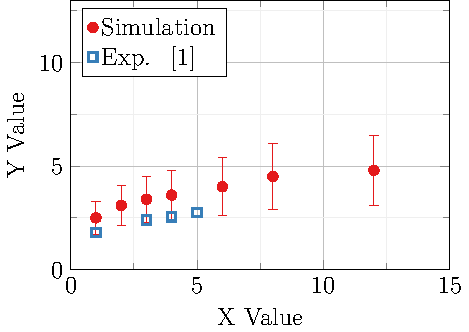
\includegraphics[width=8.6cm]{fig_1_1/fig_1_1.pdf}
  \caption{The example image with citation.}
\label{Fig:1_1}
\end{figure}


\lipsum[60]


\putbib
\end{bibunit}

% if you submit, uncomment the following and comment bibunit
% \input{../../bu1.bbl}

% =============================
% chapter2 
%%%%%%%%%%%%%%%%%%%%%%%%%%%%%%%%%%%%%%%%%%%%%%%%%%%%%%%%%%%%
% This file examplifys a chapter composed of multiple files
%%%%%%%%%%%%%%%%%%%%%%%%%%%%%%%%%%%%%%%%%%%%%%%%%%%%%%%%%%%%

\begin{bibunit}
\setcounter{chapter}{1}
\chapter{Chapter 2 Theory and Method}\label{chap:2}
\acresetall 
% abstract for chapter
\lipsum[10]

%

\section{Introduction}\label{sec:2_1}
\subsection{Intro 1}\label{subsec:2_1_1}

\lipsum[10]

\subsection{Intro 2}\label{subsec:2_1_2}

\lipsum[10]
 
%

\section{Method}\label{sec:2_2}
\subsection{Method 1}\label{subsec:2_2_1}

\lipsum[10]

\subsection{Method 2}\label{subsec:2_2_2}

\lipsum[10]
 
\putbib
\end{bibunit}

% % chap3 :: conclusion
\begin{bibunit}
\setcounter{chapter}{2}
\chapter{Conclusion}\label{chap:3}
\acresetall

\section{Summary of This Book}

\lipsum[60]


\section{Future Issues}

\lipsum[60]


\putbib
\end{bibunit}

% % appendix
\appendix
\begin{bibunit}
\chapter{Additional Simulation Results}\label{appendix:A}

% sample figure
% \begin{figure}[tbh]
 \centering
  \includegraphics[]{figA_1/Im_extinction_coef.pdf}
  \caption{Calculated imagnary part of the extinction coefficient $\eta(\omega) = 1/\varepsilon(\omega)$ for $x$ (red) and $z$ (blue) axis. The vertical dotted lines represent the energy positions of LO phonons from \cref{table:gamma} and additional peaks from \cref{fig:additional}.}
\label{fig:extinction}
\end{figure}

This is citation example~\cite{Einstein1905PE,Einstein1905SR}.
\lipsum[50]

\putbib
\end{bibunit}



\end{document}
